\chapter{Metering and Billing of Energy on Ethereum}\label{ch:implementation}

Smart contracts can transform the energy industry. In this chapter we explore the inefficiencies of the energy market and identify gaps which can be filled by blockchain. We go through the advantages of an energy-based application built on smart contracts. Finally, we describe the business logic of a specific energy use-case which we implemented on Ethereum. The implementation takes into account the methods and concepts described in Chapter \ref{ch:scalability} and Chapter \ref{ch:security} in order to ensure that the smart contracts are efficient and robust.


\section{Energy Market inefficiencies}

The global energy market is gradually transitioning to clean and renewable energy. Regulations encourage usage of distributed energy resources (DERs) \cite{europe2030}. With the integration of DERs, consumers are gradually transforming to \textit{prosumers} who store their energy surplus or sell it to their peers, effectively distributing the generation of energy, contrary to existing power systems which were designed to accommodate central points of energy generation.

There are numerous inefficiencies which need to be resolved in today's energy markets \cite{ey-inefficiencies}:
\begin{enumerate}
    \item \textbf{Transaction complexity:} More participants in the networks result in more complex transactions.
    \item \textbf{Predictability and Reliability:} Availability of DERs is less predictable compared to traditional energy resources like coal. 
    \item \textbf{Empowered prosumer:} There need be monitoring tools and infrastructure that allow prosumers to manage their energy production and consumption.
    \item \textbf{Geographic mismatches:} Locations that fully utilize DERs are usually far from key points of energy demand. Transmitting energy over long distances is inefficient.
    \item \textbf{Trust and Security:} New participants will only choose the system if it is able to be trusted and is properly secured.
\end{enumerate}

%Today's energy markets are called to resolve a number of issues.
% Having discussed how Ethereum works, and explained techniques to improve smart contracts' scalability and security, we proceed to discuss the topic of making energy markets more transparent and efficient by utilizing smart contracts. The use-case we describe can be used as a starting point for better tracking of energy usage inside a company, allowing better prediction of future needs.  
% The world is gradually shifting from nuclear and fossil fuels to Renewable Energy Sources (RES). RES have been taking a larger share of Germany's gross energy production and this has created a 
% Germany is on a rollout plan of installing smart meters in every household which incorporates RES.  
% The barrier to entry to become an energy producer\footnote{By installing solar panels for example} 
% Chart for renewables: https://www.cleanenergywire.org/factsheets/germanys-energy-consumption-and-power-mix-charts
% In its current state, most consumers do not know what they are paying Business level take long time and are 

% Price of energy, consumer does not know always what they pay, or what they gain from their renewables
 
\section{Energy Market use-cases for Blockchain}

A number of use-cases for smart contracts have been identified in the energy market. We proceed to describe applications that derive from the advantages of blockchain (transparency, trustlessness, security) as discussed in Section~\ref{advantages}.

\begin{enumerate}
    \item \textbf{Supply chain tracking and optimization:} This is a broad blockchain use case which allows for optimization on logistics and tracking the location of products, reducing fraud and ensuring the validity of an event.
    \item \textbf{Energy metering and billing:} By committing the values of energy consumed by entities to a blockchain, a timestamped record of meter readings gets generated which allows for the verification and more clear understanding of energy consumption across resources. This can be augmented to provide billing functionality (further described in \ref{business-logic}).
    \item \textbf{Peer to Peer (P2P) energy trading:} Consumers and prosumers operate in a local microgrid and trade energy between them, without a centralized operator, resulting in reduced loss of energy during transportation.
    \item \textbf{P2P Energy Micropayments:} A car that is far from its charging station is charged by the surplus energy of another car. Since this is a short-lived process that happens often, such as during the waiting time at a traffic light, in order to send and receive micropayments between the involved parties, a blockchain can be used to utilize fast payments and low transaction fees. 
    % It can also contribute to peak shaving~\footnote{Energy is billed based on the peak energy consumed during a time window. By consuming energy for charging during low peak times the peak can be reduced.} effectively reducing the costs during that time window.
\end{enumerate}

% By using smart contracts, all of the above use-cases can be automated
% Use Cases:
% - P2P Energy Trading
% - Sharing Economy - EV share and charge

% Internet of Things sensors can securely streamline inspections and repairs and automatically reduce outages.
% Applications have been developed \cite{DBLP:journals/ife/MengelkampNBDW18}

% Blockchains have the ability to provide transparency and immutability. Also,  When talking about energy and transparency, full history of meter readings, price calculation, billing of inhouse energy departments. This can be extended for EV car payment microtransactions and so on.

% The blockchain is a particularly interesting technology for decentralized processes that require large networks and trust relationships between all parties. Therefore, it offers great benefits to the power & utilities market, with its large networks of power and utilities companies, (maintenance) subtractors, (local) suppliers and end users.

% Smart meters Still, there are other applications that are ready for use in the near future. Smart meters for instance have already entered many homes. Up until now, sharing data through smart meters was a threat to the privacy of the owner of the meter. Again, the blockchain offers a potential solution. It can provide the accurate data to the supplier without requiring a direct link to the meter of specific users. When needed, the owner of the smart meter can prove to the supplier that the data are his, using his private key, and the cryptographic security of the blockchain proves that the information is accurate and hasn’t been tampered with. This puts the owner in control of his own data.

\section{Business Logic} \label{business-logic}
In collaboration with Honda R\&D Germany, we create a pilot suite of smart contracts for in-house use in order to track and bill the consumed energy of the company's headquarters as measured by a set of smart meters. 

We proceed to discuss the business logic of the use-case and then implement it. We utilize the Method 3 from Section \ref{method3} to optimize our smart contracts for gas efficiency and utilize Slither from Section~\ref{slither} and the learned best-practices to ensure that the developed smart contracts are robust. Due to the intellectual property of Honda R\&D, the contracts were tested and deployed on a private local blockchain, however it is possible to deploy the implementation to the Ethereum mainnet.

%The purpose is to serve as a means of tracking the energy consumed by the company's smart meters and ensuring the data's validity and existence in a smart contract. In addition, due to the complex structure of the company, every smart meter's consumption can contribute with different coefficients to the total energy consumption of the rooms in a building. As a result, the developed smart contract are able to track the energy consumption of each room and assign it to a higher-order 

\subsection{Metering of Energy} \label{metering}

\paragraph{Smart Meters}

A smart meter is an energy meter which sends its measured energy readings to a monitoring server for logging. A smart contract must track each smart meter by a unique identifier and store each meter's power readings, along with the time of measurement. Due to the meter not being able to \textit{ping}\footnote{Hereafter, refers to a kWh,timestamp tuple which gets stored in the blockchain.} its reading directly to the blockchain, we create a process where each the reading and timestamp of each meter is pulled from the monitoring server and then pushed to the blockchain. 

\begin{figure}[ht!]
    \centering
    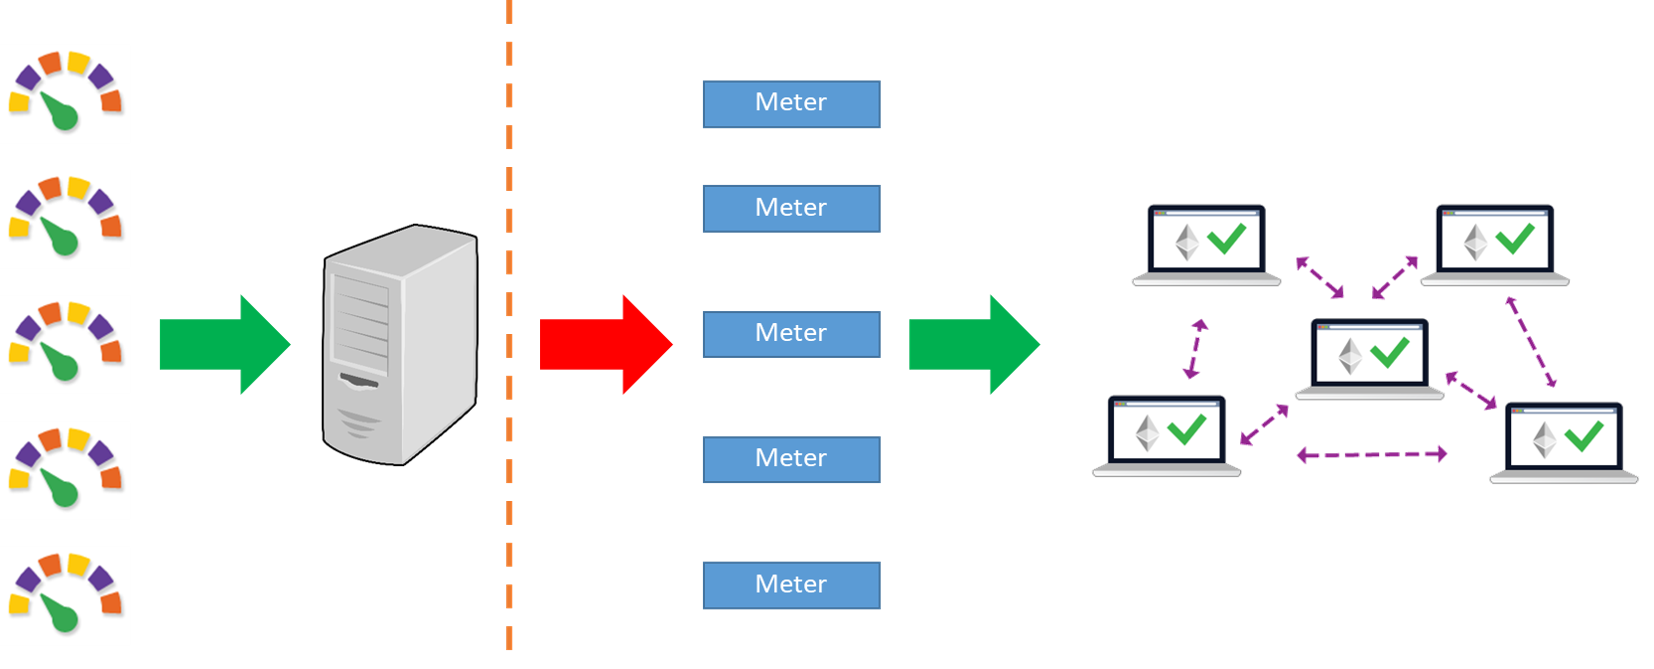
\includegraphics[width=\textwidth]{pull_push_monitoringserver}
    \caption{Meter Data gets pushed to the blockchain after getting pulled from the monitoring server}
    \label{fig:pull_push_monitoringserver}
\end{figure}
% must be able to keep track of the current reading and timestamp of the reading as well as the last reading and timestamp in order to calculate the difference of the two. It also has a unique identifier which is used to retrieve it in the smart contract.

\paragraph{Virtual Meters}

Smart meters get grouped in \textit{Virtual Meters}. The purpose of a Virtual Meter (VM) is to track the consumption of multiple Smart Meters across various rooms of a company building. As a result, the power consumption of each VM is a function of the power consumptions of its linked smart meters. % contributes to a room's consumption with a real coefficient, according to Equation \ref{roomcost}
\begin{figure}[htb]
    \centering
    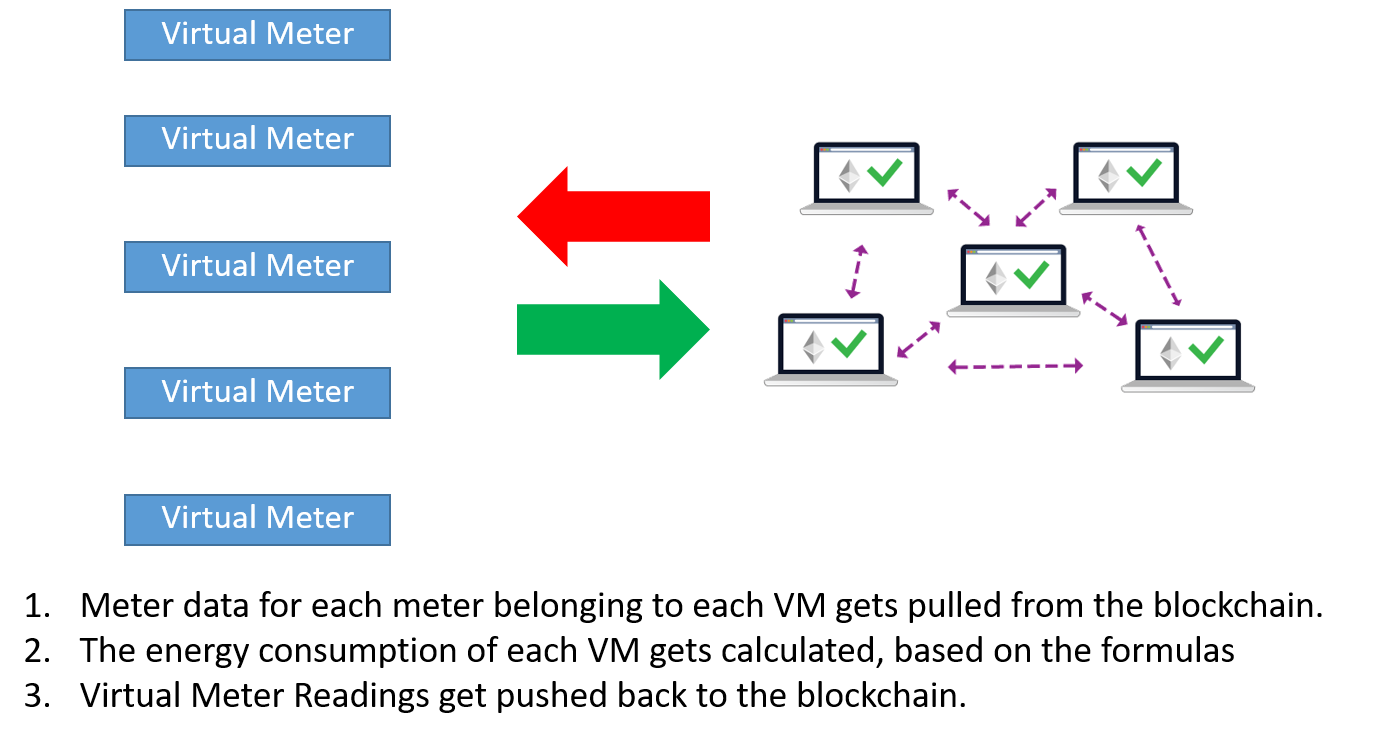
\includegraphics[width=\textwidth]{virtual_meters}
    \caption{The consumption of Virtual Meters gets calculated from the consumption of their associated Smart Meters.}
    \label{fig:virtual_meters_consumption}
\end{figure}

The formula that describes each Virtual Meter is supplied from an internal partner and is considered to be known. An example formula can be seen in Equation \ref{eq:formula}. Variables prefixed with $VM$ represent Virtual Meters, $ELT$ and $KMZ$ represent Smart Meters and $F$ represent constants.

\begin{equation} \label{eq:formula}
    \begin{aligned}
        VM15= \\
        & (ELT46-(ELT31+ELT16+ELT17+ELT35+ELT36))*F57
        \\
        + & (ELT35+ELT36-ELT18)*F27*F66
        \\
        + & (KMZ6-KMZ5)*(ELT16+ELT17+ELT18+ELT19+ELT20)\\
        & /KMZ2*F27*F66 
    \end{aligned}
\end{equation}

It is the case that this process could be done entirely on-chain, by creating a smart contract that manages virtual meters separately. This would require another smart contract for virtual meters, which would need to store the Meter IDs for each meter associated to the virtual meter, along with the formula that describes how the virtual meter consumption is calculated. This logic is unnecessarily complex to be performed on a smart contract directly. Instead, it is done off-chain on the client side, by pulling the readings of each smart meter, calculating the reading of the virtual meter, and then pushing the aggregated reading to the smart contract's storage.

\subsection{Accounting Logic} \label{billing}

\textit{Business Units} and \textit{Departments} are terms used to describe the hierarchy for the accounting business logic of the company. Business Units are used for external accounting, while departments and their subdepartments are used for internal monitoring. In implementation terms, a Business Unit is equivalent to a Department.

A Department is composed of Virtual Meters, other Departments and Delegates. Virtual Meters get grouped in Departments. A Department can include other subdepartments of a lower tier. Finally, a Department may forward its consumption to other Departments called Delegates. A department's consumption is the sum of energy consumed by its Virtual Meters, its Departments and its Delegates. 

\begin{figure}[ht!]
    \centering
    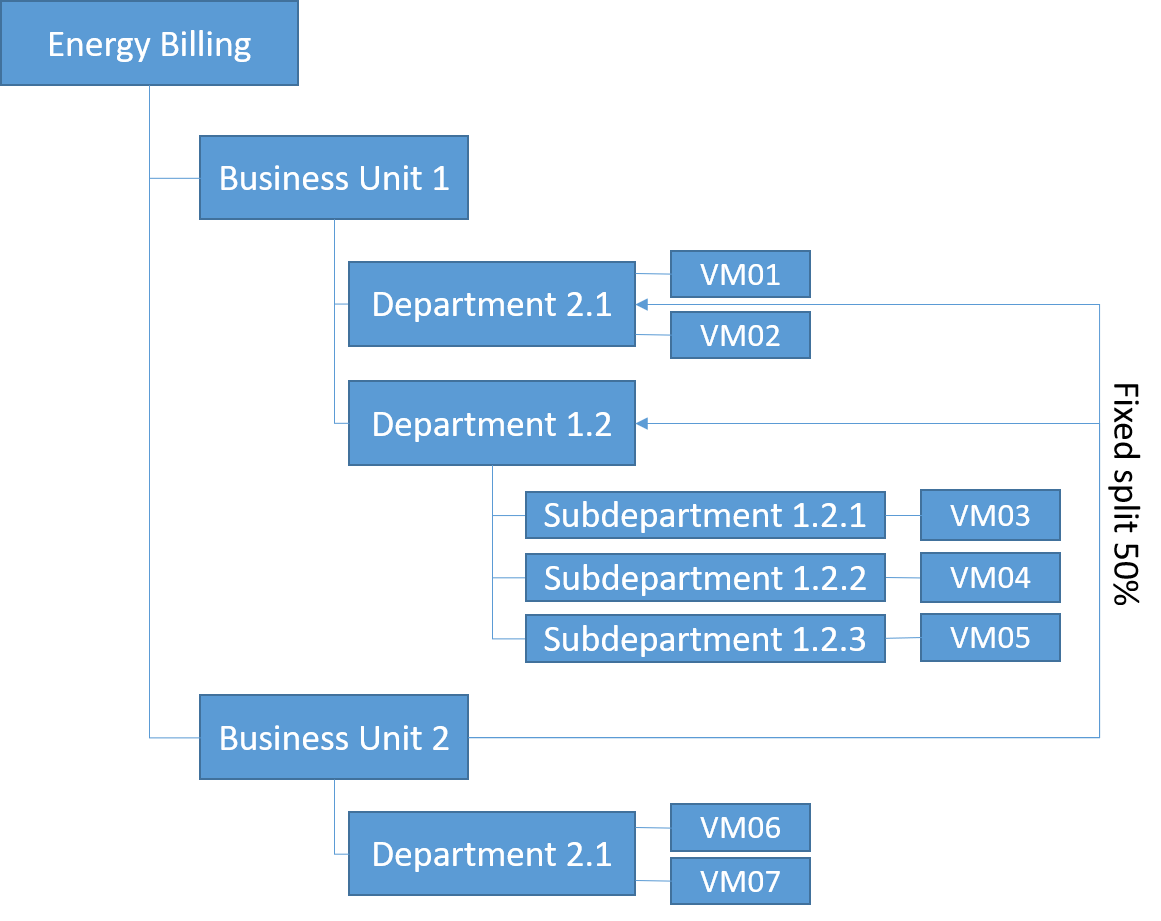
\includegraphics[width=.7\textwidth]{hierarchy}
    \caption{Relationship between Departments and Delegates.}
    \label{fig:hierarchy}
\end{figure}

Higher tier departments have the \texttt{headcount} property which defines the number of staff included in that Department. Delegation can be either through a headcount split or a fixed split. In headcount split, the amount that gets sent to each Delegate of the Department is proportional to their headcount percentage. Fixed split can only involve two Delegates, the first one receiving $X\%$ and the second one receiving $(100-X)\%$ of the Departments consumption, where $0<X<100$. As an example, in \ref{fig:hierarchy} Department 1.1 and 1.2 are fixed split delegates of Business Unit 2 and as a result their consumption is increased also by the consumption of Business Unit 2. After delegation, Business Unit 2 has its consumption cleared and will not be calculated towards the total Energy Billing.

\begin{figure}[H]
    \centering
    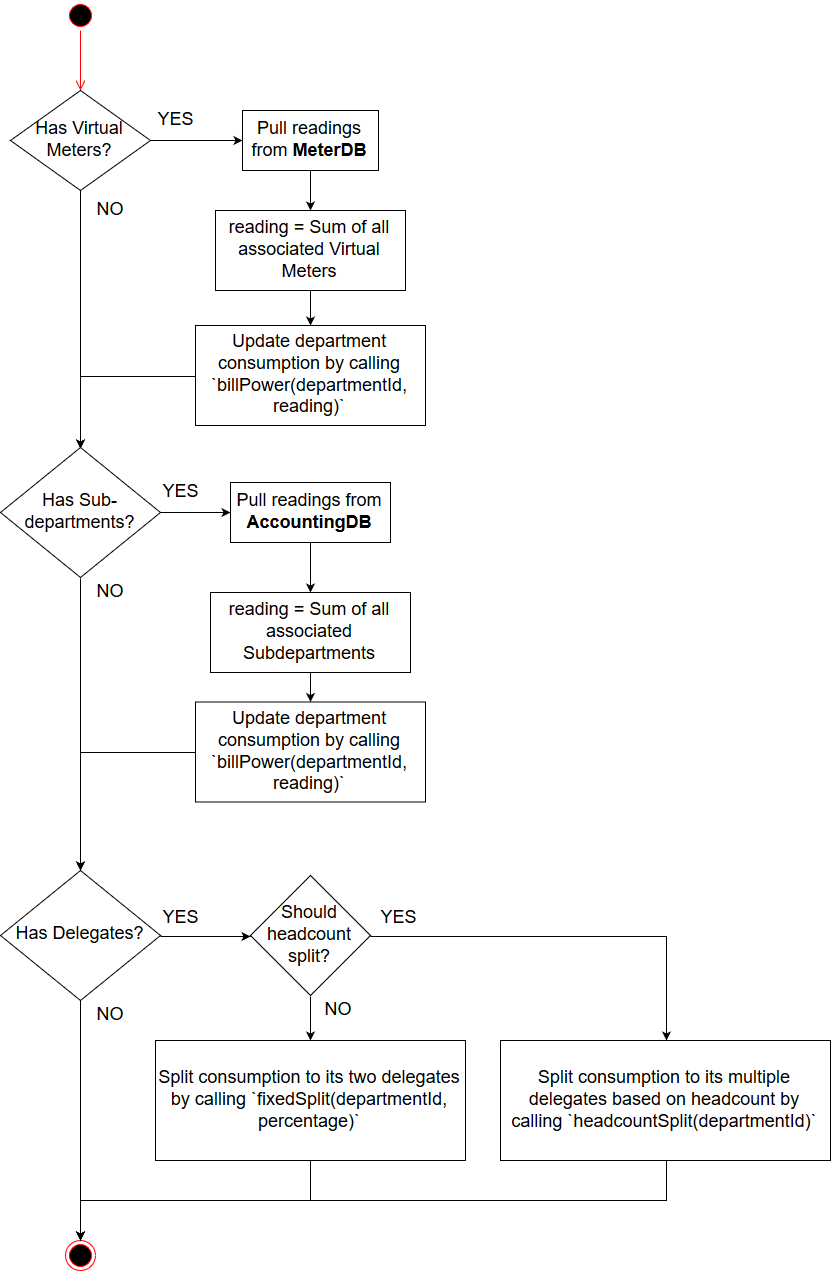
\includegraphics[width=\textwidth]{flowchart}
    \caption{Consumption calculation for a Department}
    \label{fig:consumption_flowchart}
\end{figure}

Due to the possibility of having multiple players of departments, in order to correctly calculate the final bill, the billing process starts from the inner-most tier of departments and iteratively moves outwards until the top-tier departments are reached.

\section{Smart Contracts} \label{ch:implementation:sc}
In this section we go over the implementation and the rationale of each developed smart contract. We explain the inner workings and provide tests of their functionality. We follow the design principle that the data stored on the blockchain is the minimal amount of data that needs to be trustlessly verified. Any piece of data that can be derived from the already on-chain data is generated and verified off-chain. In case data does not need to be accessed by another contract but must be transmitted to an end-user, the \texttt{Event} functionality of Solidity is used (explained in \ref{apx:ch:implementation:events}). 

\subsection{MeterDB}
MeterDB utilizes \ref{method3} to keep track of the energy consumption values and logged timestamps of a smart meter or a virtual meter. We assume that a meter can be any IoT device that has its own Ethereum account\footnote{A private-public keypair needs to be generated for every meter}. The contract is designed to map each Meter's address to its details (\texttt{id}, \texttt{reading}, \texttt{timestamp}). As a UX upgrade, a Meter's details can also be fetched by its id, if it is known. The contract is split in two files, \texttt{MeterDB.sol} which contains the business logic and \texttt{Meter.sol} which contains the logic from \ref{method3} that encodes and decodes meter data in a \texttt{bytes32} variable. It is designed intentionally to be very light for the purpose of storing and retrieving the latest readings of a meter. For each meter, its latest reading is pulled from the monitoring server and if a new consumption value has arrived it replaces the previous reading along with its timestamp by calling \texttt{ping}. Table \ref{table:meter} illustrates the design of the storage in \texttt{Meter.sol}.

\begin{table}[H]
	\centering
	\vspace*{-1ex}
	\scriptsize
	\vspace{-1ex}
	\caption{Required variables and size to describe a Meter.}
	\begin{tabular}{|c|c|c|}
        \hline
        \textbf{Name} & \textbf{Type}  & \textbf{Comment}\\ \hline 
        meterID      & bytes8         & IDs can be encoded in 8 bytes, can be optimized but hurts UX\\
        creationTime  & uint32         & Meter supports timestamps up to 2**32 = 02/07/2106 @ 6:28am (UTC) \\
        power         & uint32          & Power readings can reach up to 2**32, which is enough to store 1TWh readings \\
        \hline
    \end{tabular}
    \label{table:meter}
\end{table}
% monitoring the ID of the meter that was activated after an operator called \texttt{activateMeter}.

% A meter must be activated by an entity who has been given access to the \texttt{activateMeter} through the ACL. 

% EXPLAIN ASSUMPTIONS FOR DESIGN, NON ITERABLE BUT ITS OK. 

% Each meter has its own ID. We use the pattern. Deleting a meter sets the active status to false. We iterate over the array of meters. There are software engineering patterns \cite{crud} that allow more proper usage, however they cost a lot more gas. 

\subsection{AccountingDB}

Since part of the accounting logic is grouping \textit{Virtual Meters} in \textit{Departments} and storing the Department readings in the smart contact, there is code reuse from \texttt{MeterDB.sol}. In addition, we need to keep track of the headcount for each Department, along with its subdepartments, virtual meters, and delegates for further accounting logic. We cannot use Method 3 for encoding the accounting logic because it does not support arrays. As a result, we define two mappings for each Department, one for keeping track of the power consumption of a department and one for maintaining a list of the accounting logic associated with that department. Due to the forwarding of a department consumption to another, we keep track of the power that is generated by the virtual meters, the delegated power that is received from another department, and the cleared power which is the amount of power that has been cleared from that department, either through delegation or from accounting. 

The main addition is the forwarding logic. The forwarding can either be a \textit{Fixed Split} or a \textit{Headcount Split}. A fixed split can only be applied to a department with 2 delegates. The first delegate receives X and the second (100-X). In headcount split, for each of the sender's delegates its headcount is received and the receiver's delegated power is increased by the amount of power, proportional to the headcount. At the end, the sender's power is cleared and any further pings to that department do not consider the amount that has already been cleared. 

\begin{table}[H]
	\centering
	\vspace*{-1ex}
	\scriptsize
	\vspace{-1ex}
	\caption{Required variables and size to describe a Meter.}
	\begin{tabular}{|c|c|c|}
        \hline
        \textbf{Name} & \textbf{Type}  & \textbf{Comment}\\ \hline 
        active         & bool         & Department active flag\\
        headcount      & uint7        & Headcount percentage, between 0 and 100\\
        power          & uint80       & Power readings can reach up to 2**80\\
        delegatedPower & uint80       & Power readings can reach up to 2**80\\
        clearedPower   & uint80       & Power readings can reach up to 2**80\\
        \hline
    \end{tabular}
    \label{table:department}
\end{table}

\subsection{Access Control}
As discussed in Chapter \ref{ch:security} enforcing proper access control on critical functions of a smart contract is very important. It is common to find Access Control Lists (ACL) in enterprise environments which allow only selected participants to have to resources of various levels. This functionality does not exist by default in smart contracts. We proceed to describe the functionality of each of the mentioned roles for our smart contracts:
\begin{enumerate}
    \item Admin: Has full access to all contract functions
    \item Meter Manager: Can enable or disable a Meter at \texttt{MeterDB}.
    \item Meter: Can call the \texttt{ping} function of \texttt{MeterDB}
    \item Accountant: Can call the billing functions of \texttt{AccountingDB}
\end{enumerate}

INITIALLY ALL ACCESS CONTROL WAS DONE INSIDE EACH CONTRACT, HOWEVER IT MADE IT BIGGER TO DEPLOY BLABLA.
very light to minimize deployment costs and the costs of calling each function. A third party is able to index all the currently activated meters by monitoring the events that enabled some address to call \texttt{ping} on the ACL.

For a meter to be able to ping its reading it first needs to be activated by an authorized party, hereafter referred to as the \textit{Meter Operator}. The \textit{Meter Operator} is able to deactivate the meter, deleting its stored values from the contract. 
% The initialization of the ACL is done as shown in \ref{fig:}
% We utilize the base contract implementation of by DappSys \cite{dappsys} to create an access control list 
% The Aragon Project\footnote{Project aimed at creating DAOs} provides an ACL contract, however it was not used in the final version due to the complexity it introduced to our code\footnote{Aragon's contracts are architected towards creating fully upgradable DAOs, which would introduce considerable overheads and complexity to our code}. Instead, the DSAUTH pattern is used.

\subsection{Contract Registry} As a User Experience upgrade, a \texttt{Registry} contract was implemented. The contract links contract addresses to names through a \texttt{bytes32} to \texttt{address} mapping. The address of a contract can be changed by the registry's operator, which allows for upgradeability for contracts that refer to other contracts. As an example, a contract that calls another contract needs to know its address. Instead of modifying the destination's address in the sending contract, we go through the registry as a proxy.

ADD SHAPE. 1 - 2 - 3.

This can also be used for the client script implementations (\ref{script}) in order to reduce the number of arguments needed. Instead, the registry's address is passed to each script and they resolve each contract's name to address at runtime.

This pattern can be extended to implement further upgradeable logic, however is considered out of scope.


\section{Client Side}

We utilize Python to interact with the smart contracts and push data to them. We implement multiple command line interfaces which can be used for abstracting the complexity to an operator. The choices for each client script design are further described in Appendix \ref{apx:implementation:client}

% In order to make the code portable and ensure that the clients can be run on any machine, we also provide a Dockerfile. Docker utilizes containerization Due to design, it can be dockerized and run on multiple blabla.

% \subsection{Monitoring Server and REST API}
As mentioned in Section \ref{metering}, there is no direct access to each meter's reading. As a result, all readings are exposed through an authenticated REST API. We implement a module which gets instantiated with the Meter's Id as a parameter, and is able to interact with the monitoring server API. The primary function used is \texttt{get\_single\_reading} which fetches 1 reading from the monitoring server, by default the most recent one. In the future, the goal is to have meters which are able to send arbitrary messages over TCP/IP, which would enable this step to be skipped. 

We define a base class called \texttt{Contract} that provides functionality for interacting  with a smart contract. It allows signing offline signing of transactions and broadcasting of raw transactions which is a big security upgrade as the Ethereum node we are submitting to does not need to hold our private keys. It receives a compiled contract ABI and address to interact with the contract along with a private key for signing the transactions. The exposed function \texttt{sign\_and\_send} is used to specify which function of the contract to call, its arguments and submit it for execution to an Ethereum node.

Since these are all low level functionalities, we proceed to describe the higher level scripts which were created to provide the needed functionality of a client. All modules utilize the \texttt{Contract}, and Meter clients also use the mentioned Monitoring Server script to pull data from the REST API.

\subsection{Meter Operator}
Wrapper around \texttt{Contract}
Approves and disapproves meters.
\subsection{Single and Multiple Meters}
Uses monitoring + contract
\subsection{Single and Multiple Virtual Meters}
Uses contract and pulls / pushes. Explain AST parsing
\subsection{Accountant}
Uses 2 contracts, both meterdb and accounting, to do stuff
\subsection{Administrator}
USes the registry/ACL script to manage permissions for who can call what based on the previous things




